\documentclass[a4paper,11pt]{article}

\usepackage[utf8]{inputenc}

\usepackage{graphicx}
\usepackage{caption}
\usepackage{subcaption}

\usepackage{pgfplots}
\usepackage{float}
\usepackage{hyperref}
\usepackage{soul}
\hypersetup{
    colorlinks=true, % Enable colored links
    linkcolor=black, % Color for internal links
    urlcolor=black,  % Color for external links
    citecolor=black, % Color for citation links
    pdfborder={0 0 0}, % Remove border around links
}
\newcommand{\underlinehref}[2]{%
    \href{#1}{\ul{#2}}%
}
\pgfplotsset{compat=1.18}


\usepackage{minted}

\begin{document}

    \title{
        \textbf{Sorting Arrays in C}
    }
    \author{Péter Herczku}
    \date{Fall 2024}

    \maketitle

    \section*{Introduction}

    The task is to analyze the time complexity of different sorting algorithms in particular selection, insertion and merge-sort.
    I completed the assignment using the C programming language.

    \section*{Swapping elements in an array}

    Since we will swap elements in multiple algorithms, it would be convenient to create a {\tt swap} method that does the job for us.

    \begin{minted}{c}
void swap(int* array, int index1, int index2) {
    int temp = array[index2];
    array[index2] = array[index1];
    array[index1] = temp;
}
    \end{minted}

    \section*{Selection sort}

    The simplest sorting algorithm that is pretty straightforward to implement is selection sort.
    The idea behind it is the following: we start from index 0 and look for the smallest element in the array that is smaller than our value at index 0.
    We swap them, increment index by one, and we keep doing the same thing until we reach the end of the array.
    In the worst case, we do $n^2/2$ comparisons, therefore this algorithm should have $O(n^2)$ time complexity.
    First let's take a look at the implementation of selection sort:

    \begin{minted}{c}
void sort(int* array, int length) {
    for (int i = 0; i < length - 1; i++) {
        int candidate = i;
        for(int j = i + 1; j < length; j++) {
            if (array[j] < array[candidate]) {
                candidate = j;
            }
        }
        swap(array, i, candidate);
    }
}
    \end{minted}
    Now, let's run some benchmarks to validate our point about the time complexity of selection sort.

    \begin{figure}[h]
        \centering
        \begin{subfigure}[b]{.5\textwidth}
            \centering
            \includegraphics[width=\textwidth]{./selection/data} % Adjust width or height as needed
        \end{subfigure}
        \caption{Graph of selection sort}
        \label{fig:graph_1}
    \end{figure}

    We can clearly see the quadratic relationship from the graph: if we double the size of the array, the runtime will be multiplied by 4.

    \subsection*{Insertion sort}

    This algorithm is a bit trickier to implement than selection sort, but we still shouldn't have any problems programming it.
    We start from index 1, and we start going backwards.
    If the value of the element at the target index is bigger than our value at the current index we swap them.
    We keep doing this until we reach the beginning of the array, or we reach an element that is smaller than ours.
    After that, we increment index by one and do the same thing until we reach the end of the array.
    Now, let's look at the implementation of the function:

    \begin{minted}{c}
void sort(int* array, int n) {
    for (int i = 1; i < n; i++) {
        for (int j = i - 1; j >= 0 && array[j] > array[j + 1]; j--) {
            swap(array, j, j + 1);
        }
    }
}
    \end{minted}
    In the worst case, it should still be an algorithm with $O(n^2)$ time complexity.
    However, when the array is partially sorted the algorithm should perform better than selection sort, but since we are working with large randomized arrays this is negligible.
    After running some benchmarks, we get the following result:

    \begin{figure}[h]
        \centering
        \begin{subfigure}[b]{.5\textwidth}
            \centering
            \includegraphics[width=\textwidth]{./insertion/data} % Adjust width or height as needed
        \end{subfigure}
        \caption{Graph of insertion sort}
        \label{fig:graph_2}
    \end{figure}

    We can observe a quadratic relationship from the graph again, but luckily we can do better.
    Let's discuss it in the next topic.

    \subsection*{Merge sort}

    \begin{figure}[h]
        \centering
        \begin{subfigure}[b]{.5\textwidth}
            \centering
            \includegraphics[width=\textwidth]{./merge/data} % Adjust width or height as needed
        \end{subfigure}
        \caption{Graph of merge sort}
        \label{fig:graph_3}
    \end{figure}

\end{document}
